\section{Methods}

\subsection{Modified Rankin Scale}

Modified Rankin Scale (mRS) is the most commonly used instrument to describe post-stroke functional outcome \cite{quinn_functional_2009}. Table \ref{tab:mrs} shows a description of the seven level so f mRS along with utilties, from Wang \emph{et al.}\cite{wang_utility-weighted_2020}. Utilities are a measure of the preference or value that an individual or society gives a particular health state, with 1 being full health and 0 being dead (values of less than zero describe states where death is considered preferable).

\begin{minipage}{\textwidth}
\renewcommand*{\arraystretch}{2.0} % adjust row spacing
\begin{longtable}[]{@{}llr@{}}
\caption{A description of modified Rankin Scale score, with Utilities from Wang \emph{et al.}\cite{wang_utility-weighted_2020}}\\
\toprule
mRS & Description. & Utility\tabularnewline
\midrule
\endhead
0 & No symptoms. & 0.97\tabularnewline
1 & No significant disability: Able to carry out all usual activities,
despite some symptoms. & 0.88\tabularnewline
2 & \makecell[l]{Slight disability: Able to look after own affairs without assistance, but unable to carry \\ out all previous activities.} &
0.74\tabularnewline
3 & Moderate disability: Requires some help, but able to walk
unassisted. & 0.55\tabularnewline
4 & \makecell[l]{Moderately severe disability: Unable to attend to own bodily needs without assistance, \\ and unable to walk unassisted.} & 0.20\tabularnewline
5 & Severe disability: Requires constant nursing care and attention,
bedridden, incontinent. & -0.19\tabularnewline
6 & Dead. & 0.00\tabularnewline
\bottomrule
\label{tab:mrs}
\end{longtable}
\end{minipage}

\subsection{General model description}

\Anna{Check consistency of our names for "no effect time" and other prob dists.}

\Anna{How will we write log(odds ratio) and similar? "log of odds ratio", "logarithmic odds ratio"...? Wait for the copy editor to invent something worse...?}

% mRS distribution derivation

We define outcome in terms of probability distributions of mRS scores. 
\Anna{add description of mRS dists here}


% Probability with time:
% Words description:
We use these outcome probability distributions to model the variation of outcome probability with time \sout{for each combination of occlusion type and treatment}.
% 
For a given mRS category $x$ at time $t$, the probability values, $P(\mRS\leq x\ |\ t)$, can be converted to odds, $O(\mRS\leq x\ |\ t)$, and \logodds, $\log_e[O(\mRS\leq x\ |\ t)]$, by using the standard definition $O=P/(1-P)$.
The \logodds\ can be modelled similarly to outcome \logoddsratio, which falls off approximately linearly with time\cite{emberson_effect_2014, fransen_time_2016}. 
% 
The known relation between \logodds\ and time can then be converted back into relations for odds and probability with time.

% Maths description:
We define a straight line fit $\log_e[O(\mRS\leq x\ |\ t)] = A_x + b_x t$
for constants $A_x$ and $b_x$ that differ for each mRS category $x$, $0\leq x \leq5$.
This gives an exponential form of odds where $O(\mRS\leq x\ |\ t) = \exp{(A_x + b_x t)}$.
The conversion to probability uses the inversion of the standard relation between probability and odds,  $P=O/(1+P)$. 
The final result is probability in the form of a logistic function:

\begin{equation}
P(\mRS\leq x\ |\ t) = \frac{1}{1+\exp{(A_x + b_x t)}}
\end{equation}


The constants $A_x$ and $b_x$ are found by considering the known data at $t=0$ and $t=\tne$. 
When $t=0$ then $A_x = \log_e[O(\mRS\leq x\ |\ t=0)]$ and when $t=\tne$ then $b_x = (\log_e[O(\mRS\leq x\ |\ t=\tne)] - A_x) / \tne$. 

The resulting distributions of probability with time are given in Figure~\ref{fig:probs_with_time} for each combination of occlusion type and treatment method. \checkthis{Do we want a table?} The constants $A_x$ and $b_x$ for each case are given in Table~\ref{tab:probs_with_time} \Anna{which we could always banish to an online supplement.}

% Table for A and b:
\begin{table}
    \centering
    \begin{tabular}{rrrrrrr}
        \hline 
        & nLVO IVT & & LVO IVT & & LVO MT & \\
        mRS ($x$) & $A_x$ & $b_x$ & $A_x$ & $b_x$ & $A_x$ & $b_x$ \\ 
        \hline 
        0 & ? & ? & ? & ?  & ? & ? \\
        1 & ? & ?  & ? & ?  & ? & ? \\
        2 & ? & ?  & ? & ?  & ? & ? \\
        3 & ? & ?  & ? & ?  & ? & ? \\
        4 & ? & ?  & ? & ?  & ? & ? \\
        5 & ? & ?  & ? & ?  & ? & ? \\
        6 & ain't none & nah & ? & ? & ? & ? \\
        \hline
    \end{tabular}
    \caption{\Anna{Do we want a table like this?} $\mRS\leq x$}
    \label{tab:probs_with_time}
\end{table}

\begin{figure}
    \centering
    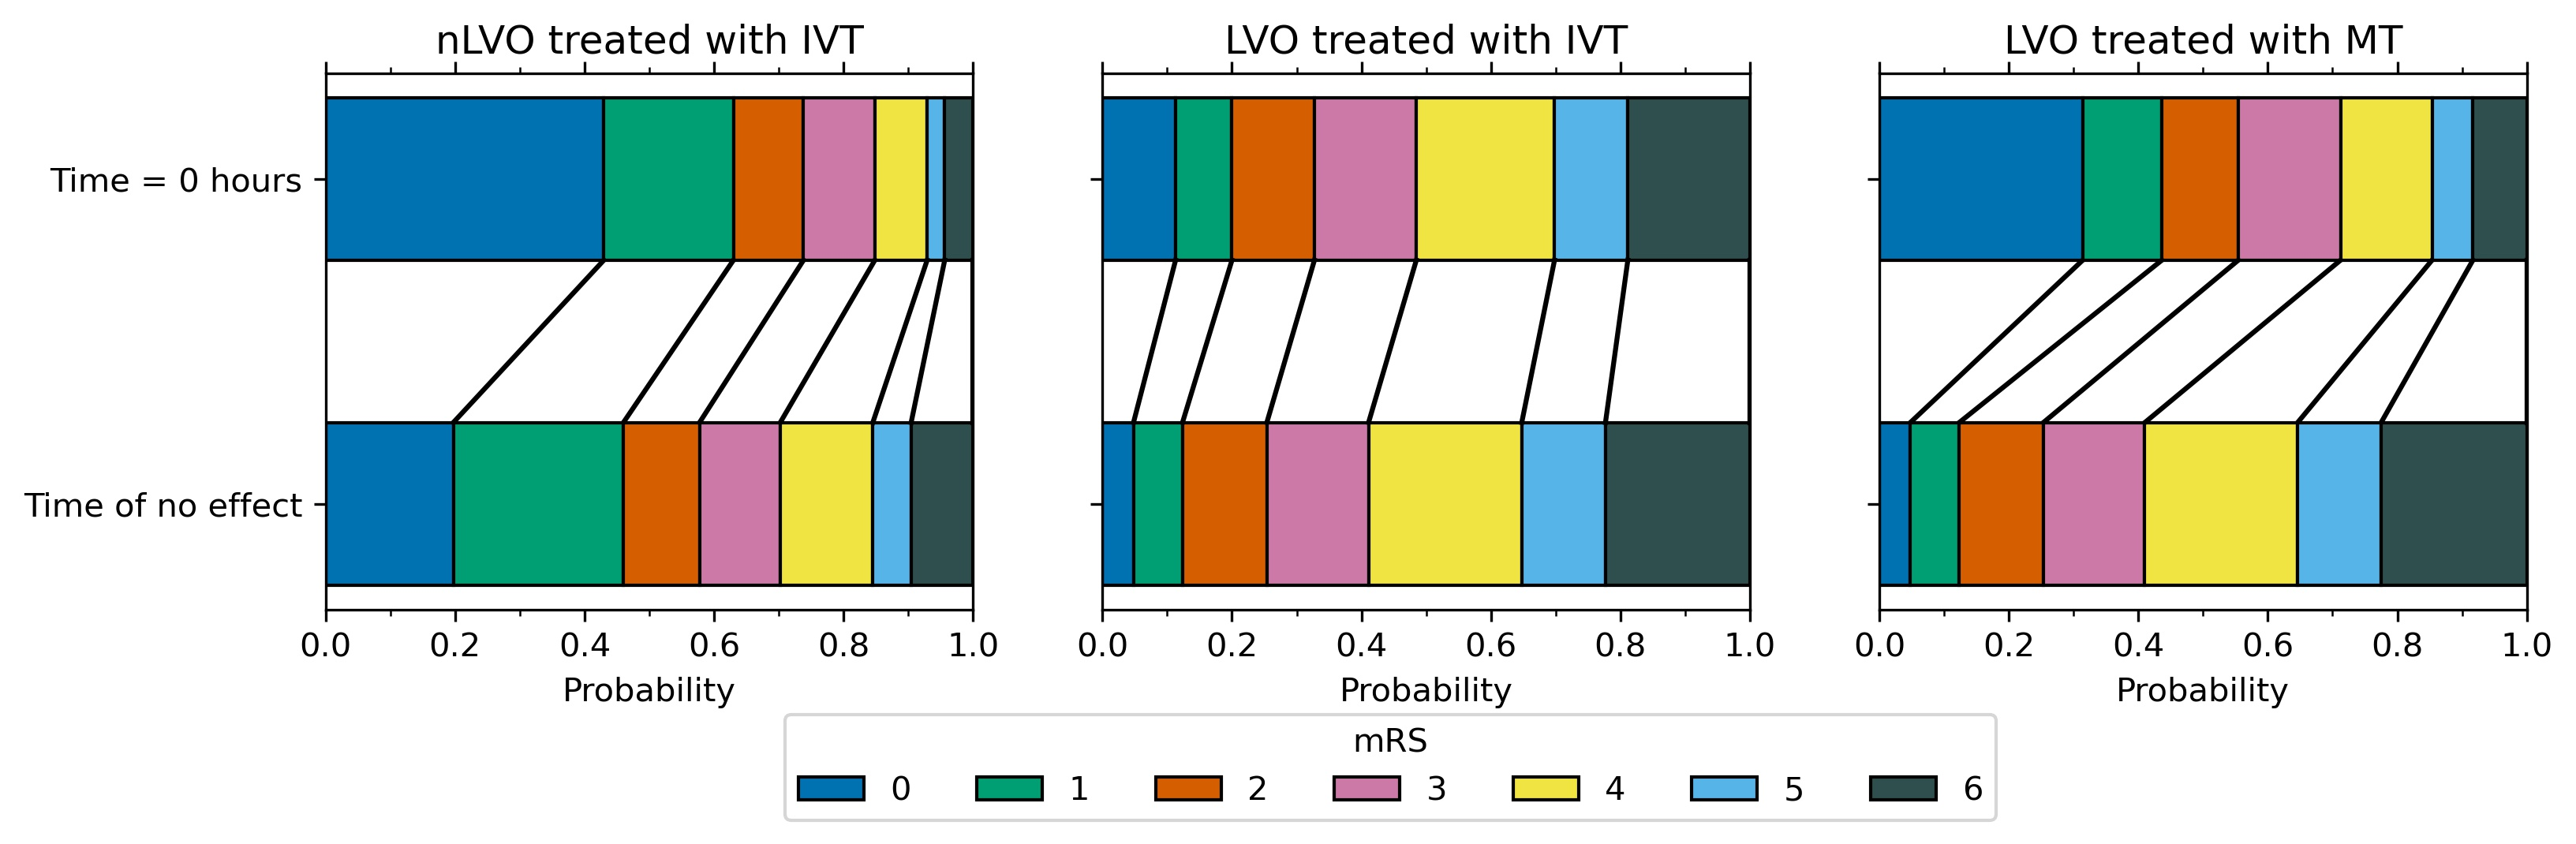
\includegraphics[width=\columnwidth]{images/dist_bars.jpg}
    \caption{
        The probability distributions of the mRS values of different patient populations. 
        The data sources and derivations \checkthis{are explained in the text...?}.
        The values associated with each distribution are tabulated in Table~\ref{}. \checkthis{presumably? Or they can be plonked onto the figure.}
        }
    \label{fig:dist_bars}
\end{figure}

\begin{figure}
    \centering
    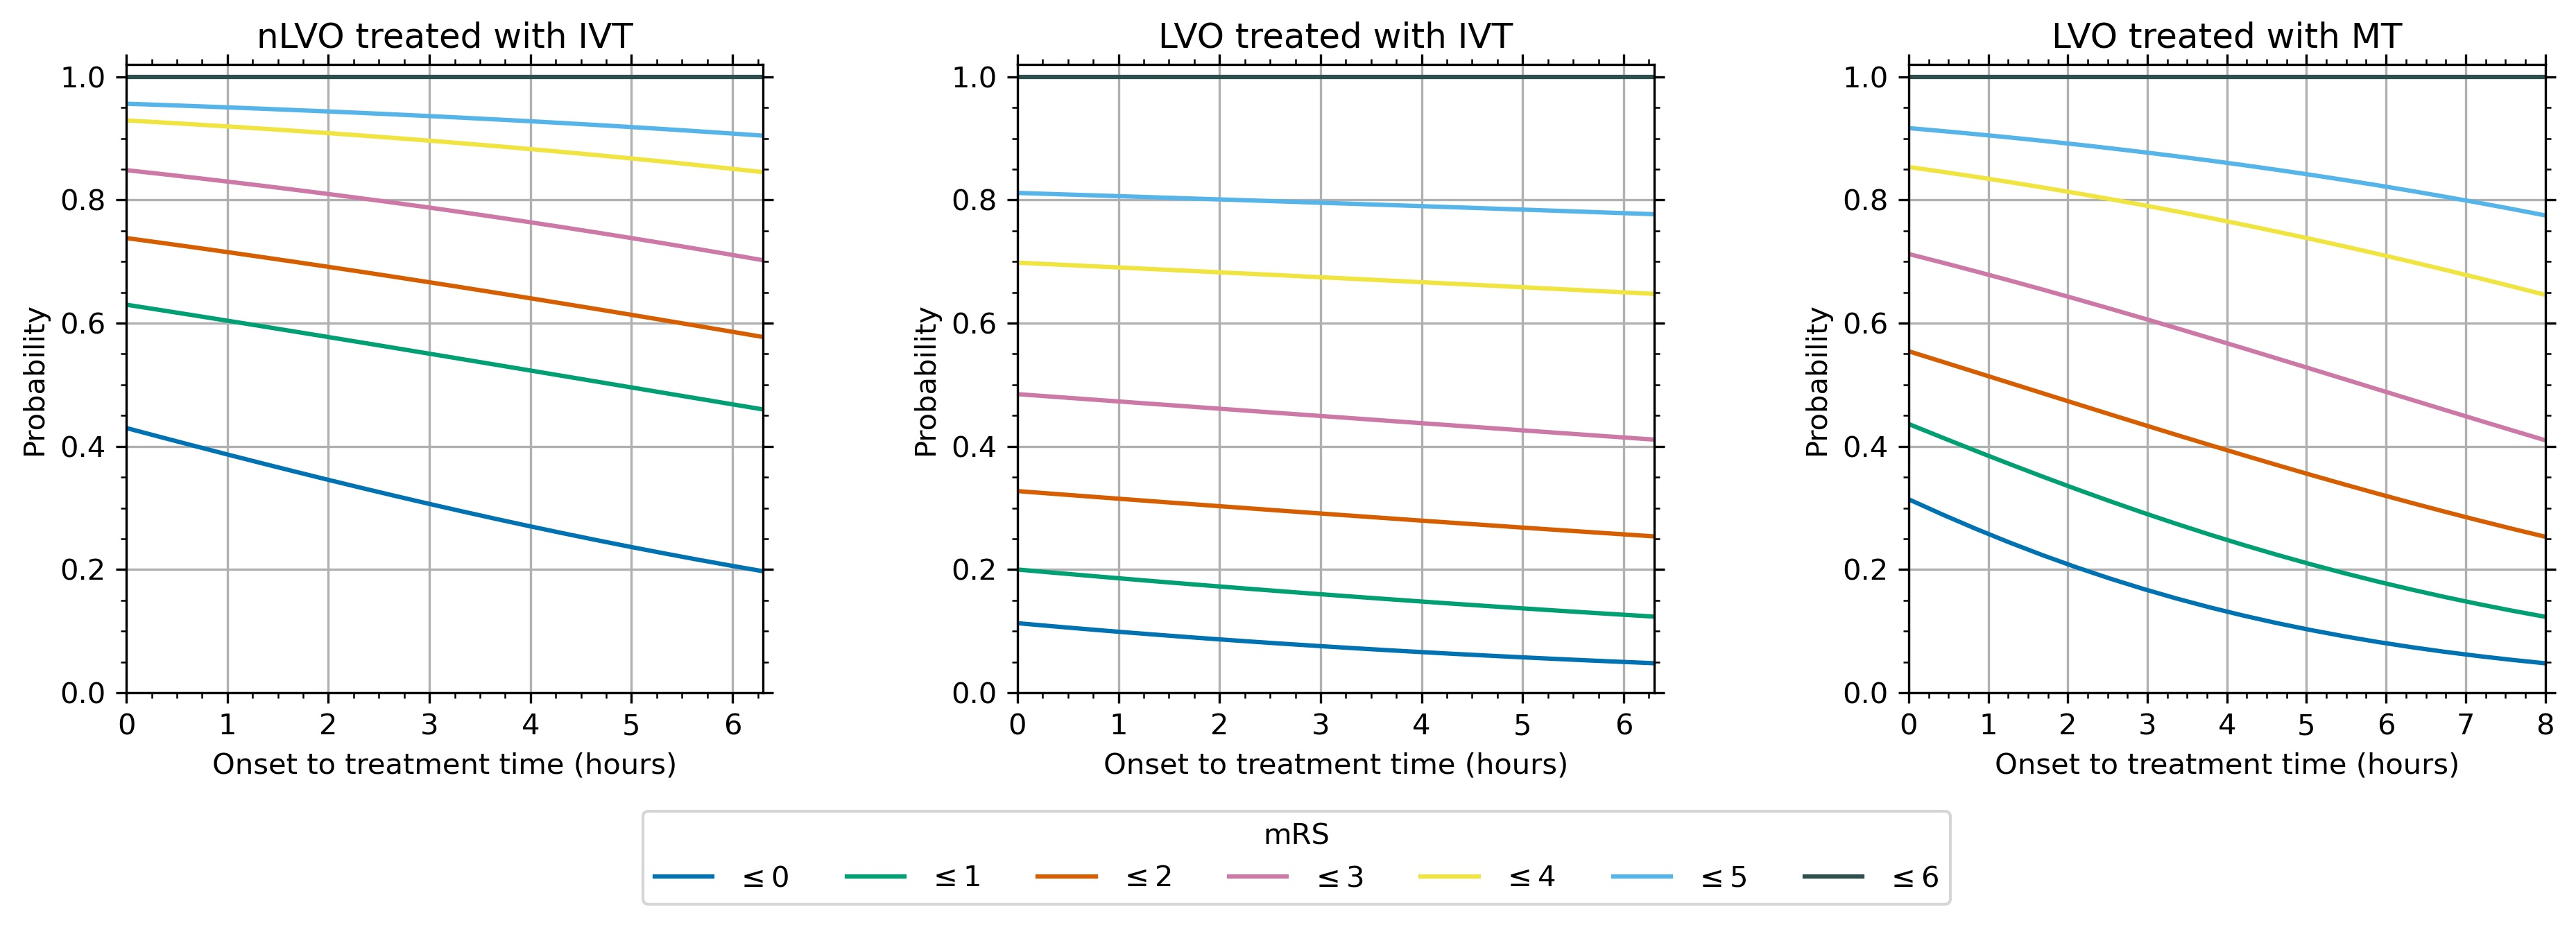
\includegraphics[width=\columnwidth]{images/probs_with_time.jpg}
    \caption{
        The variation of the mRS probability distributions with time.
        The maximum times shown are the times-of-no-effect, which for IVT is 6.3\,hr \cite{emberson_effect_2014},
        and for MT is 8.0\,hr\cite{goyal_endovascular_2016}\checkthis{check source}.
        }
    \label{fig:probs_with_time}
\end{figure}

\begin{figure}
    \centering
    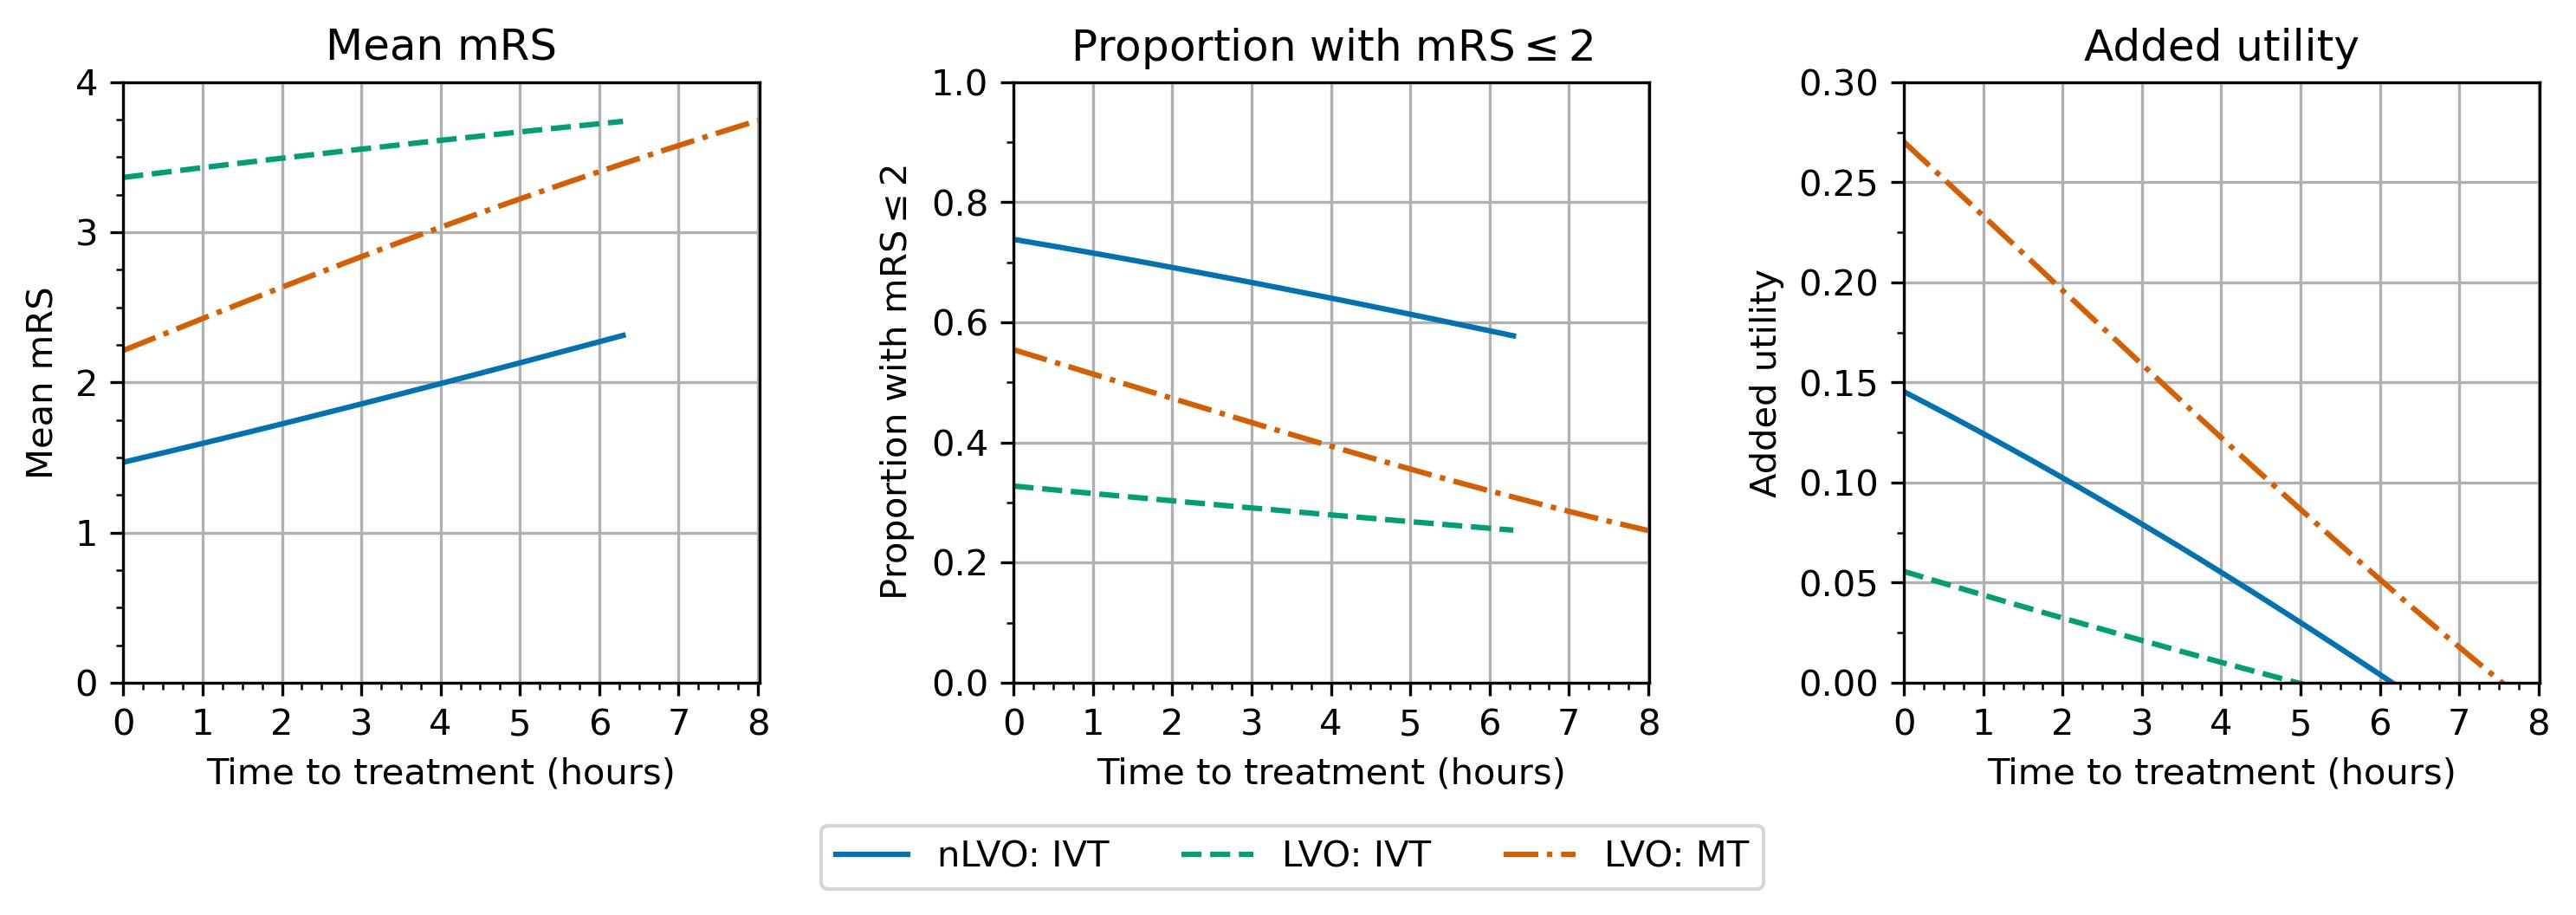
\includegraphics[width=\columnwidth]{images/time_to_treatment.jpg}
    \caption{
        The various outcomes for a representative patient population when the whole population has the same onset-to-treatment time and is given the treatment type. 
        \checkthis{should right-hand panel y-axis go below zero?}
        }
    \label{fig:changes_with_time}
\end{figure}


\begin{figure}
    \centering
    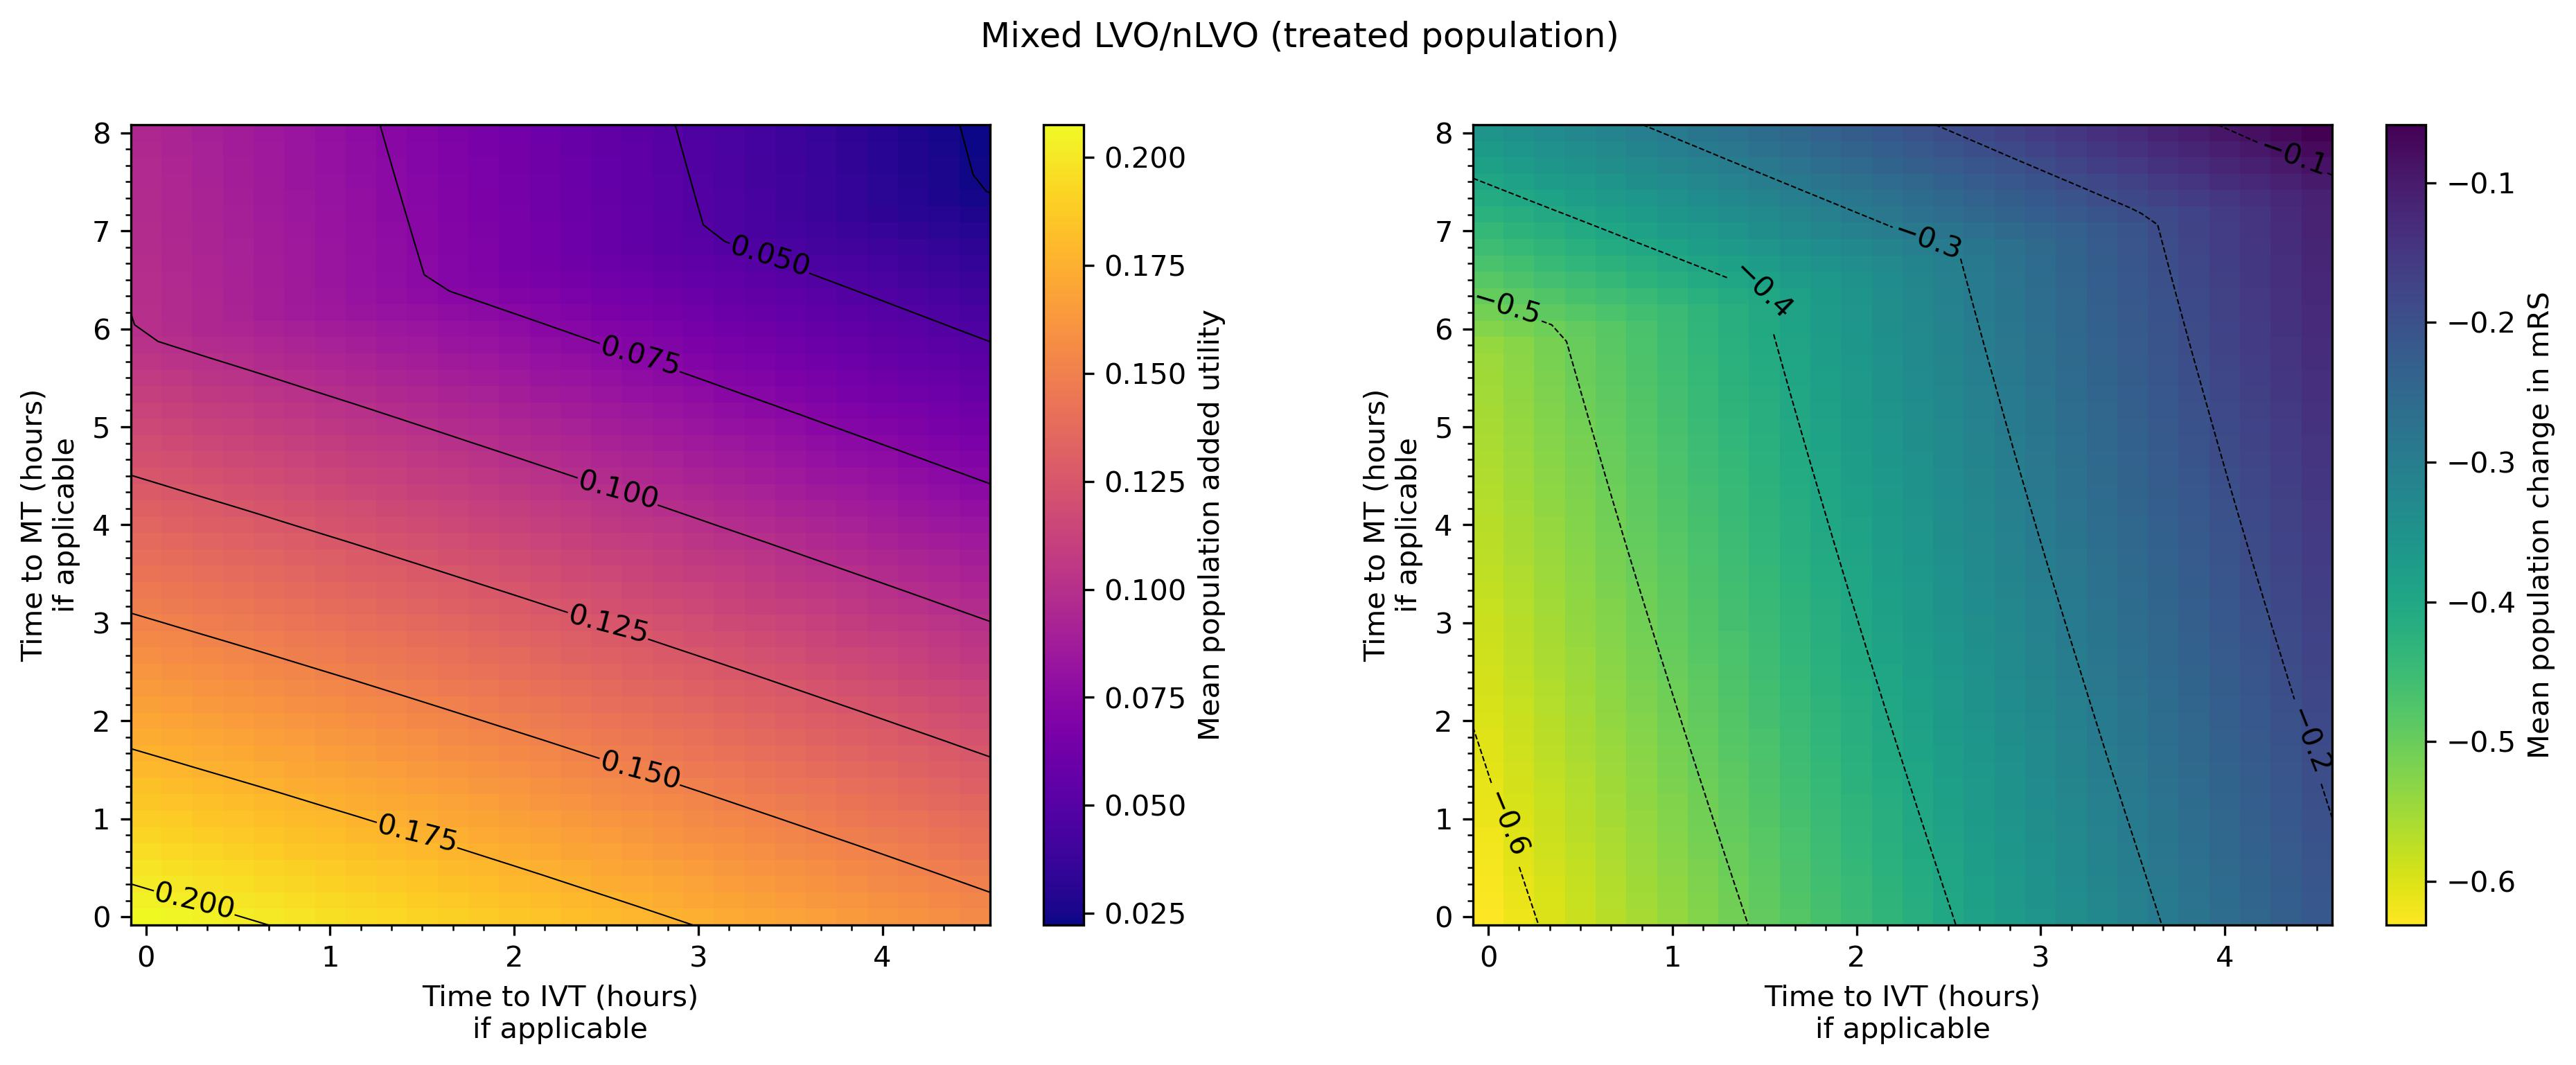
\includegraphics[width=\columnwidth]{images/matrix_utility_and_mRS.jpg}
    \caption{
        The expected mean change in utility (left panel) and mRS (right panel) for a representative patient population. At each combination of time to IVT and time to MT, every person in the population is given the treatments that they are eligible for. Larger resulting mean improvements are shown in paler colours.
        \checkthis{Why does the IVT time go up to 4.something hours when usually we use 6.3?}
        }
    \label{fig:matrix}
\end{figure}


\begin{figure}
    \centering
    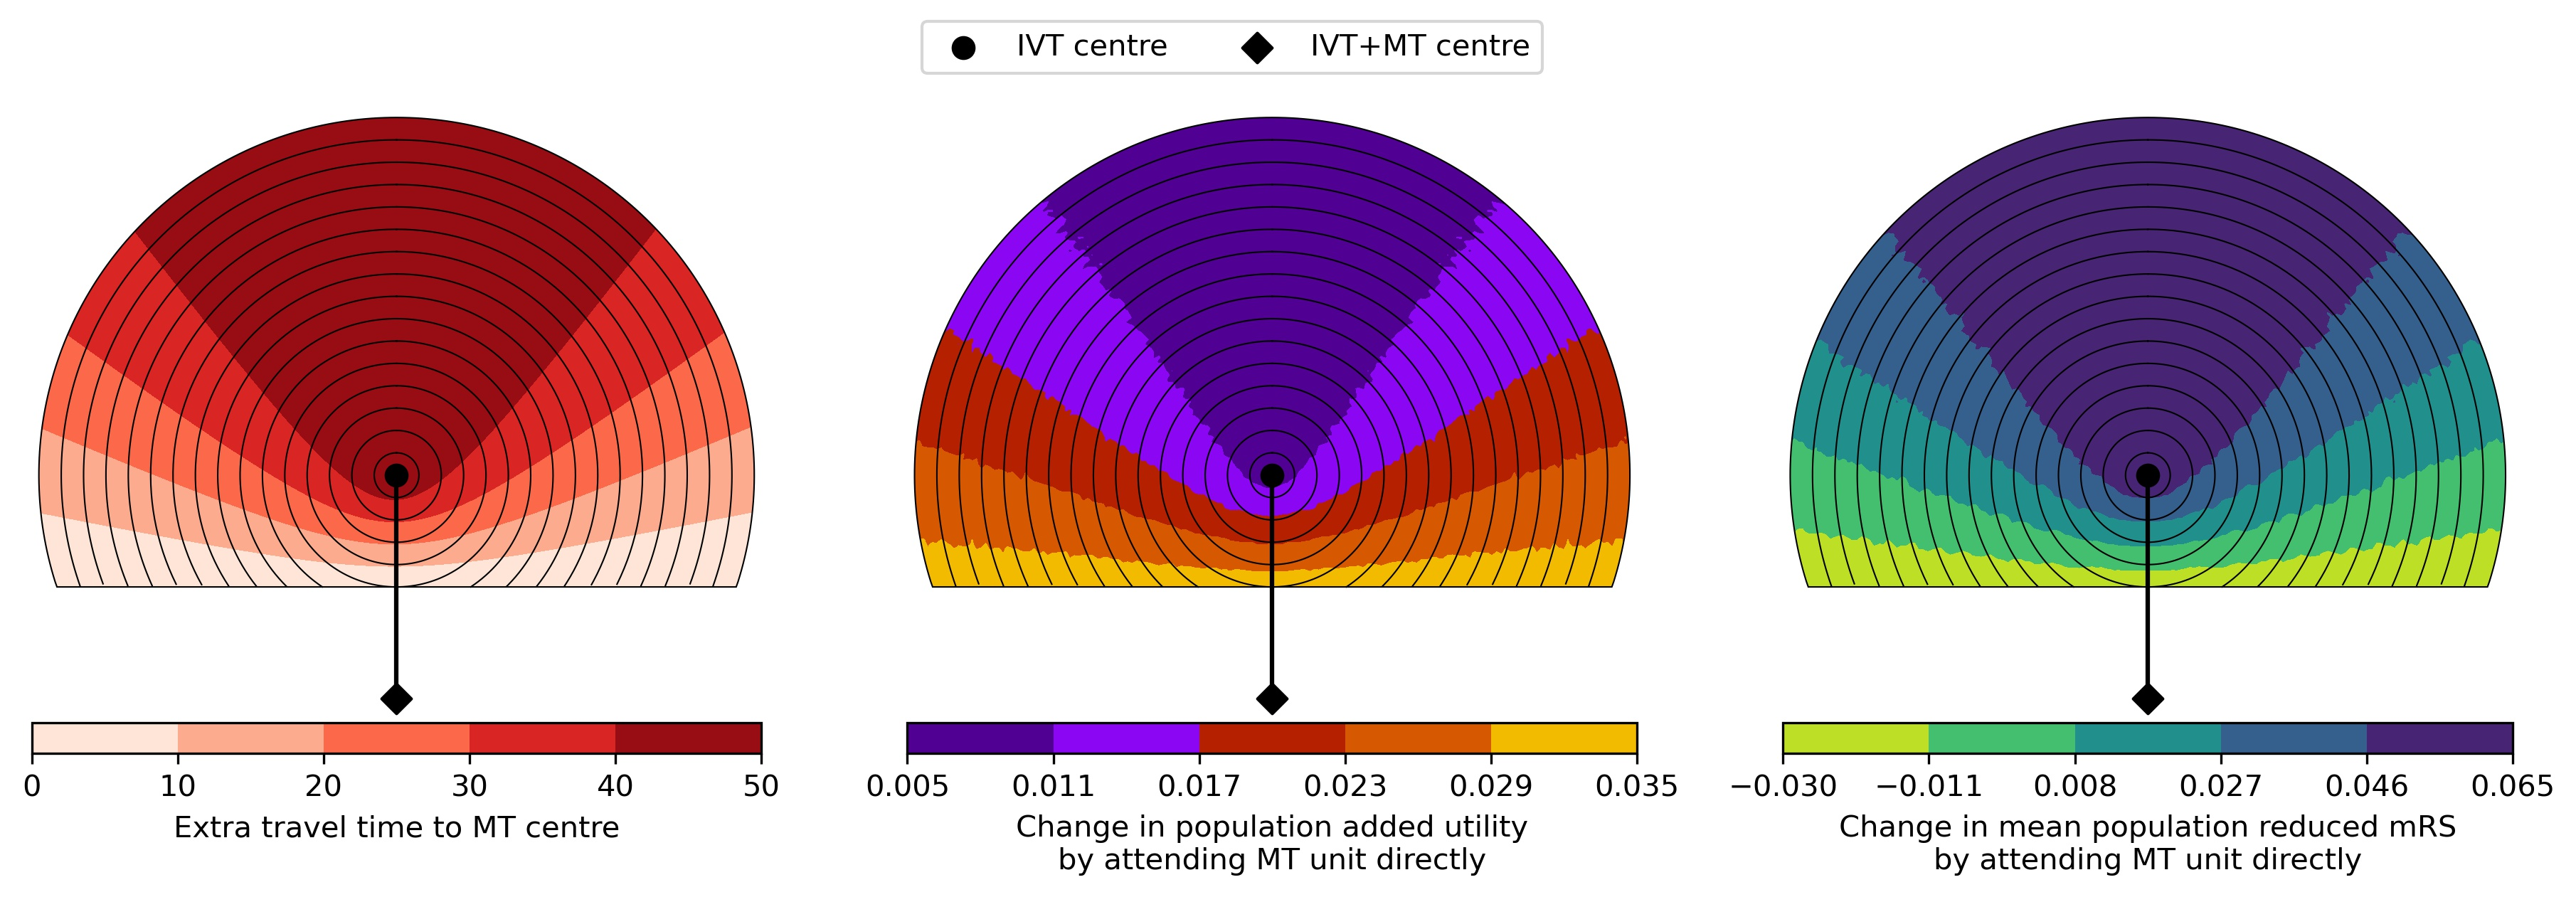
\includegraphics[width=\columnwidth]{images/circle_plots.jpg}
    \caption{
        The effect of extra travel time between treatment centres on the expected outcome of a representative patient population.
        The concentric circles represent five-minute intervals \checkthis{check} of travel time from the IVT-only centre
        and are only shown in regions where the IVT-only centre is closer than the IVT+MT centre. 
        The left panel shows only the extra travel time to the IVT+MT centre, and the middle and right panels show the effect of the increased travel time on utility and mRS respectively. 
        c.f. previous geographic modelling  \cite{holodinsky_modeling_2018}. 
        }
    \label{fig:circles}
\end{figure}
